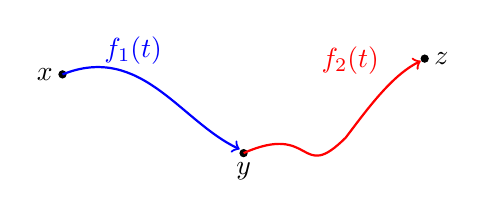
\begin{tikzpicture}
  \fill (0,1) circle (1.5pt) node[left] {$x$};
  \fill (2.3,0) circle (1.5pt) node[below] {$y$};
  \fill (4.6,1.2) circle (1.5pt) node[right] {$z$};
  \draw[->, thick, blue] (0,1) .. controls (1.0,1.4) and (1.5,0.4) .. (2.25,0.05) node[pos=0.35, above] {$f_1(t)$};
  \draw[->, thick, red] (2.3,0) .. controls (3.2,0.4) and (3.0,-0.4) .. (3.6,0.2) .. controls (3.9,0.6) and (4.2,1.0) .. (4.55,1.17) node[pos=0.6, above left] {$f_2(t)$};
\end{tikzpicture}
